\chapter{Implémentation pratique}

\section{Introduction}

Dans ce chapitre, nous présentons la réalisation pratique de notre projet. Après avoir étudié et simulé les différentes méthodes de commande dans l'environnement MATLAB, nous passons à l'implémentation sur le système réel. Cette étape consiste à mettre en œuvre la commande neuronale sur une carte ESP32 et à établir la communication avec une deuxième carte chargée de l'acquisition des données du système thermique à l'aide du capteur DHT22. Nous décrivons aussi les différents composants utilisés, l'architecture du système ainsi que les résultats expérimentaux obtenus.

\section{Architecture matérielle}

\subsection{Carte de développement ESP32}

L'ESP32 est un microcontrôleur puissant et peu coûteux, bien adapté à notre projet, fabriqué par la société Espressif Systems. Nous avons choisi cette carte car elle intègre un module Wi-Fi et Bluetooth. On a utilisé l'ESP32 pour piloter le système et assurer une connexion sans fil.

\begin{figure}[H]
	\centering
	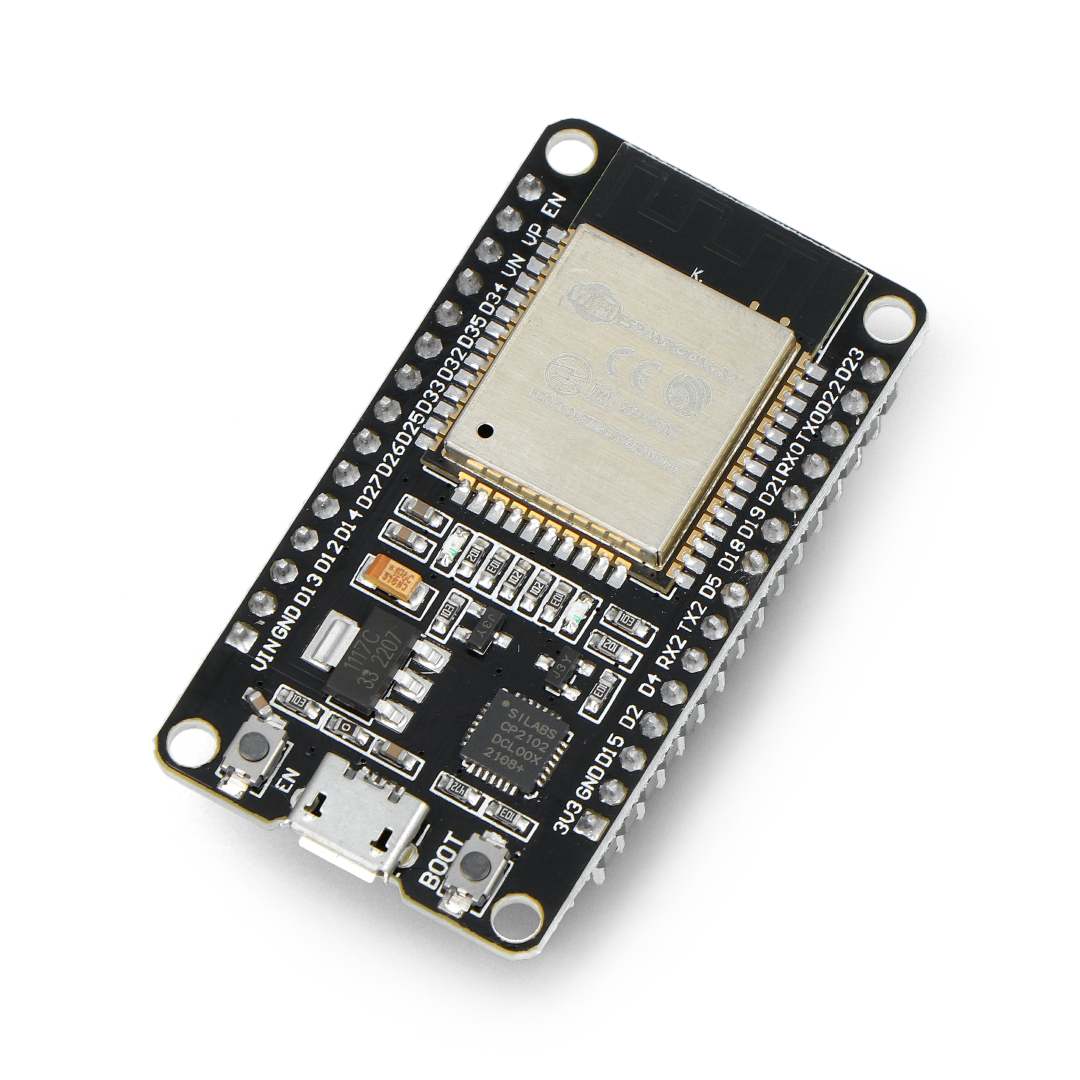
\includegraphics[width=0.4\linewidth]{figures/esp.jpg}
	\caption{Le microcontroleur ESP32}
	\label{fig:esp32_carte}
\end{figure}

\vspace*{0.5 cm}

Ses principales caractéristiques sont présentées dans le tableau suivant :

\begin{table}[H]
	\centering
	\caption{Extraits du datasheet du microcontroleur ESP32}
	\begin{tabular}{|l|l|}
		\hline
		\textbf{Caractéristique} & \textbf{Description} \\ \hline
		Microcontrôleur & ESP32 (double cœur) \\ \hline
		Fréquence CPU & Jusqu'à 240 MHz \\ \hline
		Mémoire RAM & 520 KB SRAM \\ \hline
		Mémoire Flash & 4 MB \\ \hline
		Connectivité & Wi-Fi 802.11 b/g/n, Bluetooth v4.2 \\ \hline
		Tension de fonctionnement & 3.3 V \\ \hline
		Entrées/Sorties GPIO & Jusqu'à 34 broches \\ \hline
		ADC (Convertisseur analogique-numérique) & 12 bits \\ \hline
		DAC (Convertisseur numérique-analogique) & 2 canaux \\ \hline
		Interfaces de communication & UART, SPI, I2C, CAN \\ \hline
		Consommation & Faible consommation (mode veille disponible) \\ \hline
	\end{tabular}
\end{table}

\subsection{AC Dimmer Module}

Le module AC Dimmer (Gradateur) est un contrôleur de puissance pour charges alternatives (AC) 220~V, utilisant une technologie TRIAC à coupure de phase. Compatible avec Arduino/ESP32, il gère 1 canal (8~A) via une logique 3.3~V/5~V, détecte le passage par zéro pour une variation précise (lumière, moteurs). On a utilisé ce module pour contrôler l'intensité d'une lampe.

Les pins du module AC Dimmer :

\begin{itemize}[label=$\bullet$]
	\item \textbf{VCC} et \textbf{GND} : pour l'alimentation du module.
	\item \textbf{Z-C} : permet de détecter le passage par zéro de la tension du secteur. Elle génère un signal numérique à chaque fois que la tension alternative atteint 0 V, ce qui permet au microcontrôleur de se synchroniser avec le réseau électrique. Cette synchronisation est essentielle pour assurer une commande précise du TRIAC et réduire les perturbations électriques.
	\item \textbf{PSM} : utilisée pour recevoir le signal de commande (MLI) provenant de l'ESP32. Ce signal permet de contrôler la puissance fournie à la charge en ajustant le moment de déclenchement du TRIAC après le passage par zéro.
\end{itemize}

\begin{figure}[H]
	\centering
	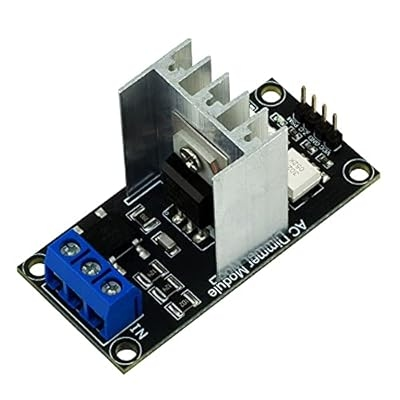
\includegraphics[width=0.3\linewidth]{figures/dimmer.jpg}
	\caption{Module actionneur à Triacc (Dimmer)}
	\label{fig:dimmer_module}
\end{figure}

\subsection{Capteur de température DHT22}

Le DHT22 est un capteur numérique utilisé pour mesurer la température et l'humidité de l'air. Dans notre projet, il est utilisé pour mesurer la température du système thermique et envoyer les données à la carte ESP32 pour le traitement et la commande.

\begin{figure}[H]
	\centering
	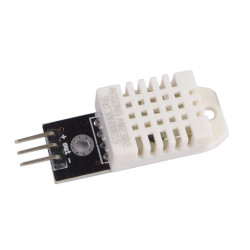
\includegraphics[width=0.3\linewidth]{figures/dht.jpg}
	\caption{Capteur d'humidité et de température DHT22}
	\label{fig:dht22_capteur}
\end{figure}

\begin{table}[H]
	\centering
	\caption{Caractéristiques du capteur DHT22}
	\begin{tabular}{|l|l|}
		\hline
		\textbf{Caractéristique} & \textbf{Valeur / Description} \\ \hline
		Type de capteur & Température et humidité \\ \hline
		Plage de température & $-40^\circ$C à $+80^\circ$C \\ \hline
		Précision température & $\pm0.1^\circ$C \\ \hline
		Plage d'humidité & 0\% à 100\% RH \\ \hline
		Précision humidité & $\pm2$ à 5\% RH \\ \hline
		Tension d'alimentation & 3.3 V à 5 V \\ \hline
	\end{tabular}
\end{table}

\subsection{Equipement de chauffage 220V}

On utulise comme effecteur de chauffage pour le systéme une lampe 220 V, pour varier la température dans une boîte fermée. Elle est efficace car elle reçoit une puissance importante du module Dimmer.

\section{Architecture du système}

L'architecture générale du système thermique est représentée par la figure suivante :

\begin{figure}[H]
	\centering
	\begin{tikzpicture}[
		box/.style={draw, rectangle, minimum width=2cm, minimum height=0.8cm, align=center, font=\small},
		arrow/.style={-{Stealth[length=3mm]}, thick},
		]
		
		%% Boîte fermée
		\draw[thick] (5,1.5) rectangle (10,6.5);
		\node[anchor=north west, font=\small] at (5,6.5) {Boîte fermée};
		
		%% DHT22
		\node[box] (dht22) at (7.5,5.5) {DHT22};
		
		%% Lampe
		\draw[thick] (7.1,2.8) rectangle (7.9,3.4);
		\draw[thick] (7.5,3.4) circle (0.45);
		\node[anchor=west, font=\small] at (8.1,3.2) {Lampe};
		
		%% ESP32 droite (mesure)
		\node[box, minimum width=2cm] (esp32R) at (3,0) {ESP32\\mesure};
		
		%% ESP32 gauche (commande)
		\node[box, minimum width=2cm] (esp32L) at (0,0) {ESP32\\commande};
		
		%% Dimmer
		\node[box, minimum width=2cm] (dimmer) at (7.5,0) {Dimmer};
		
		%% 220 V
		\node[font=\normalsize, anchor=west] (v220) at (10.5,0) {220~V};
		
		%% Flèches
		\draw[arrow] (esp32R.west) -- node[above, font=\small] {mesure} (esp32L.east);
		\draw[arrow] (esp32L.south) -- ++(0,-0.6) -| node[below, pos=0.25, font=\small] {commande} (esp32R.south);
		\draw[arrow] (esp32R.east) -- node[below, font=\small] {commande} (dimmer.west);
		\draw[arrow] (dimmer.east) -- (v220.west);
		
		%% DHT22 → ESP32 mesure
		\draw[arrow] (dht22.south) -- (7.5,4.5) -- (3,4.5) node[midway, above, font=\small] {mesure} -- (esp32R.north);
		
		%% Dimmer → Lampe
		\draw[thick] (7.5,0.4) -- (7.5,1.5) -- (7.5,2.8);
		
	\end{tikzpicture}
	\caption{Schéma synoptique du système de régulation thermique}
	\label{fig:schema_systeme}
\end{figure}

Le système est composé de deux cartes ESP32 qui communiquent entre elles sans fil. La première carte est utilisée pour mesurer la température du système thermique à l'aide du capteur DHT22 et envoyer ces données à la deuxième carte. La deuxième carte reçoit les informations, exécute l'algorithme de commande basé sur les réseaux de neurones et calcule l'action de commande. Cette action est ensuite envoyée vers un module dimmer AC qui contrôle la puissance appliquée à une lampe 220~V, permettant ainsi de réguler la température du système. Cette architecture permet de séparer l'acquisition des données et le traitement de la commande pour assurer que l'utilisateur contrôle le système à distance.

\subsection{Essai en boucle ouverte}

Tout d'abord, dans le cadre de notre travail pratique, nous avons commencé par réaliser un essai en boucle ouverte sur le système thermique, où une commande constante notée $u$ a été appliquée sur des intervalles de 2000 échantillons, avec un échantillonnage toutes les 2 secondes grâce au capteur DHT22. Les températures mesurées ont été sauvegardées dans le but de créer une base d'apprentissage, qui nous sert ensuite à entraîner un réseau de neurones artificiels utilisé sur une carte ESP32, dont les poids sont indispensables à la mise en œuvre de notre algorithme de commande à minimum de variance. De cette manière, nous avons non seulement appris à comprendre le comportement du système mais aussi préparé la phase de commande intelligente.

Les données enregistrées après l'essai en boucle ouverte sont présentées dans la figure suivante.

\begin{figure}[H]
	\centering
	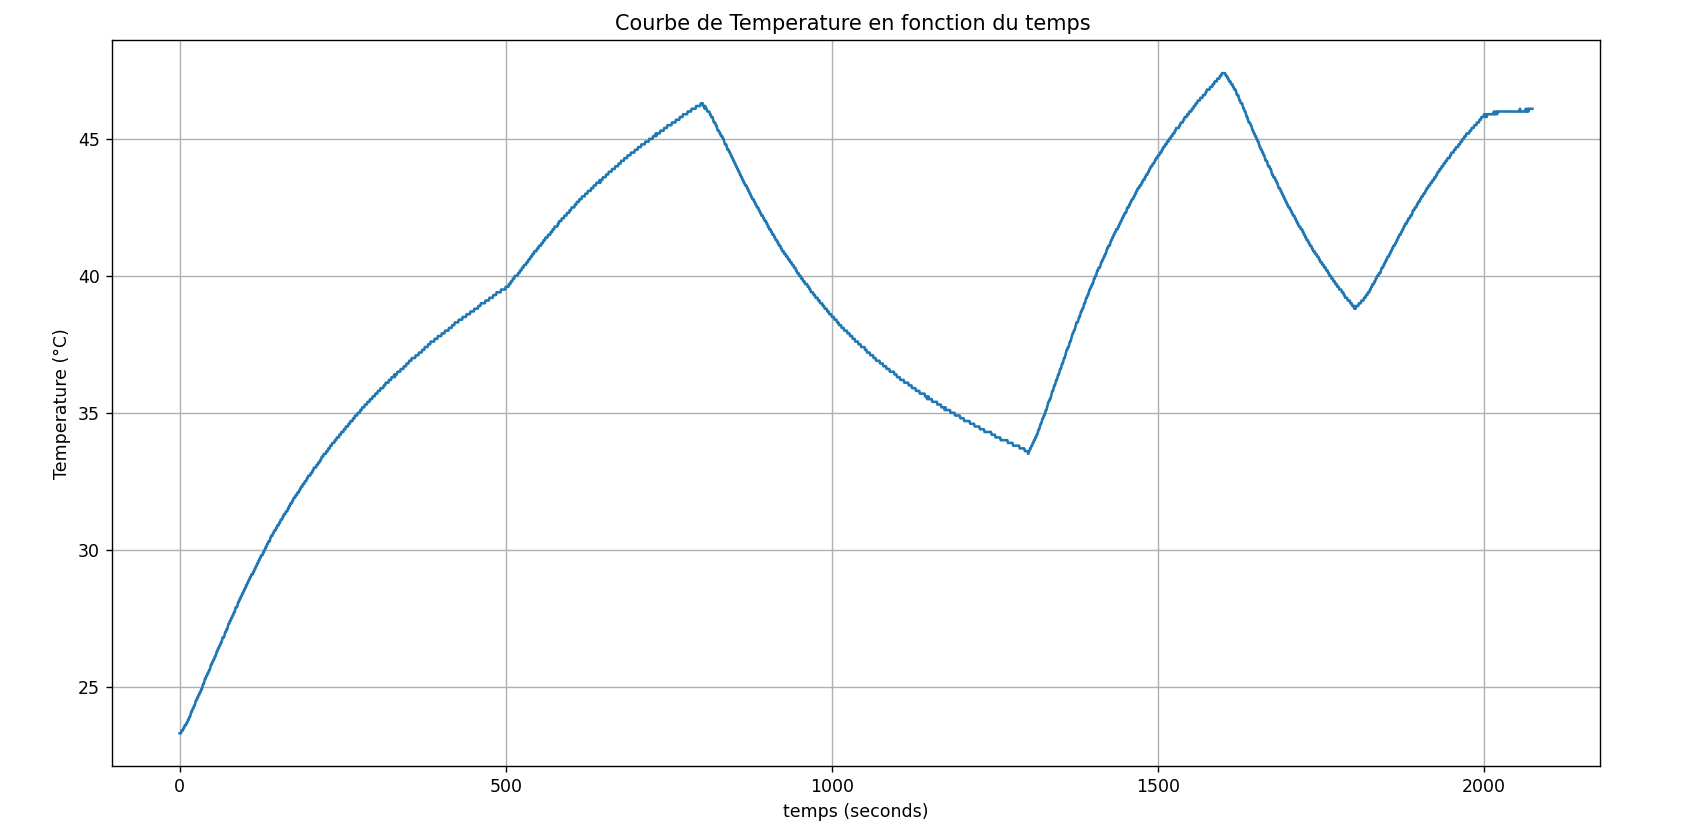
\includegraphics[width=1\linewidth]{figures/temperature.png}
	\caption{Evolution de la température en fonction du temps}
	\label{fig:temperature}
\end{figure}

\section{Apprentissage du neurone artificiel}

Dans cette partie, nous avons utilisé les données obtenues lors de l'essai en boucle ouverte pour entraîner un neurone artificiel. Ces données, qui représentent l'évolution de la température en fonction de la commande appliquée, ont été traitées sous MATLAB pour constituer un jeu d'apprentissage. Ensuite, un algorithme d'apprentissage a été mis en place pour ajuster les poids du neurone afin de minimiser l'erreur entre la sortie réelle et la sortie estimée. Les résultats obtenus sont présentés sous forme de figures dans les sections suivantes, afin d'analyser la qualité de l'apprentissage et la capacité du modèle à reproduire le comportement du système thermique.

Tout d'abord, nous avons ouvert les fichiers qui contiennent les données enregistrées et avons parcouru ces valeurs pour les stocker dans un vecteur. Les valeurs de température ont été divisées par 100 pour les normaliser entre 0 et 1. Cela facilite le processus d'apprentissage et améliore la stabilité de l'algorithme.

Ensuite, nous avons initialisé les variables nécessaires à l'apprentissage, comme les poids du neurone et les paramètres de l'algorithme. Nous avons également introduit les valeurs de la commande $u$, utilisées lors de l'essai en boucle ouverte, et les avons normalisées en les divisant par 5. Cela nous permet d'avoir des données d'entrée cohérentes avec celles de sortie.

Après cela, nous avons mis en œuvre l'algorithme principal d'apprentissage. Cet algorithme ajuste les poids du neurone de manière itérative pour minimiser l'erreur entre la sortie réelle du système et la sortie estimée par le modèle.

Une fois l'apprentissage réalisé, une phase de test qui suit permet de valider encore l'efficacité du modèle choisi.

Enfin, les résultats de simulation sont affichés sous forme de courbes. Cela nous permet de visualiser la qualité de l'apprentissage et la précision du modèle. Ces figures montrent la capacité du neurone à reproduire le comportement du système thermique.

\begin{figure}[H]
	\centering
	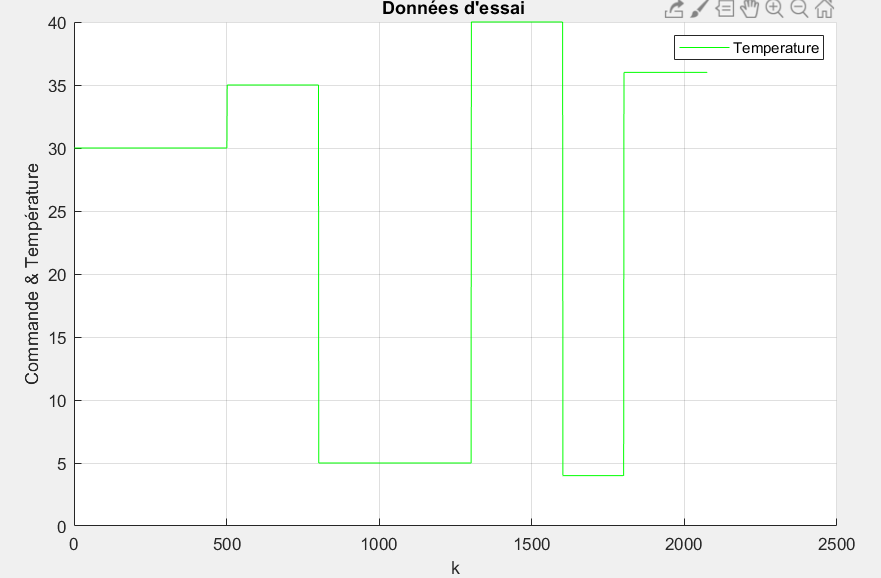
\includegraphics[width=1\linewidth]{figures/Command_Boucle_Ouverte}
	\caption{Évolution de la commande en puissance  pendant  l'essai en boucle ouverte}
	\label{fig:commandboucleouverte}
\end{figure}

\begin{figure}[H]
	\centering
	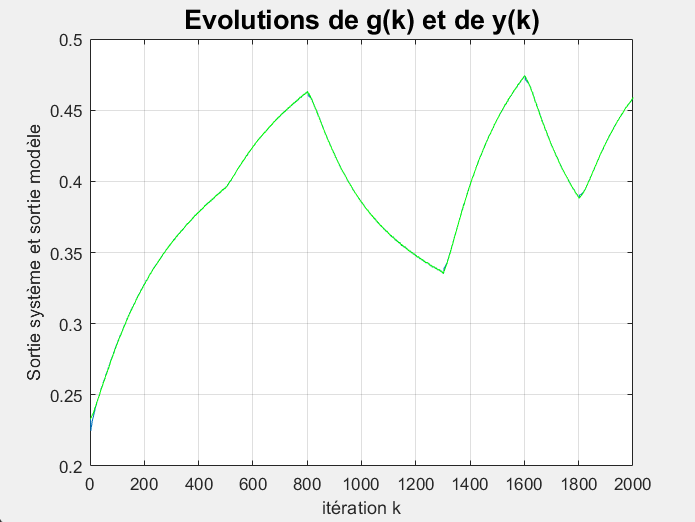
\includegraphics[width=0.90\linewidth]{figures/resultatapprent.png}
	\caption{Évolution de la sortie système et de la sortie prédite du neurone pendant l'apprentissage}
	\label{fig:apprentissage}
\end{figure}

\begin{figure}[H]
	\centering
	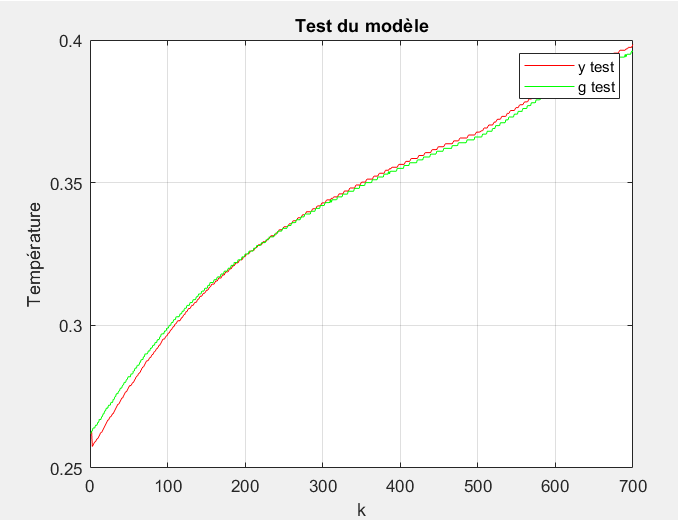
\includegraphics[width=0.90\linewidth]{figures/resultattest.png}
	\caption{Évolution de la sortie système et de la sortie prédite du neurone pendant le test}
	\label{fig:test_neurone}
\end{figure}

\section{Essai en boucle fermée}

Après la phase d'apprentissage, nous passons à un essai en boucle fermée en utilisant une commande à minimum de variance. Cet algorithme de commande exploite les poids obtenus lors de l'apprentissage du neurone artificiel afin d'estimer le comportement du système et de calculer l'action de commande optimale. Ainsi, le système devient capable d'ajuster automatiquement la puissance appliquée pour suivre la consigne de température tout en minimisant l'erreur et les variations indésirables.

\subsection{Implémentation de l'algorithme sur la carte}

Dans cette étape, nous avons mis en œuvre l'algorithme de commande à minimum de variance sur la carte ESP32. Cet algorithme utilise les poids que nous avons obtenus lors de la phase d'apprentissage du neurone artificiel pour estimer le comportement du système et calculer la commande à appliquer.

\begin{itemize}[label=$\bullet$]
	\item \textbf{RBDdimmer} : cette bibliothèque donne des fonctions prédéfinies pour contrôler le dimmer.
	\item \textbf{DHT} : permet de lire les valeurs de température mesurées par le capteur DHT22 avec la fonction prédéfinie \texttt{dht.readTemperature()}.
\end{itemize}

Le programme sur la carte ESP32 est conçu de manière simple pour fonctionner en temps réel. Tout d'abord, il initialise les variables et configure les entrées et les sorties ainsi que les communications nécessaires. Ensuite, le programme lit la température mesurée par le capteur DHT22. Il utilise les poids du neurone ($w_0$, $w_1$, $w_2$, $w_3$ et $w_4$) obtenus lors de la phase d'apprentissage pour calculer la commande. Cette commande est ensuite envoyée au module de puissance dimmer pour contrôler le système thermique. Une boucle infinie répète ces étapes en continu pour réguler la température.

\subsection{Montage expérimental}

La broche \textbf{data} du capteur DHT22 transmet la valeur de la température à la carte ESP32. Cette dernière calcule ensuite la commande de contrôle. Elle attend ensuite le signal de synchronisation provenant de la broche \textbf{Z-C} du dimmer, puis envoie la commande via la broche \textbf{PSM}. Le dimmer module alors la puissance issue du secteur et l'applique à la lampe, ce qui modifie la température dans la boîte isolée. Ce cycle se répète en continu afin d'assurer la régulation et de permettre à la température de suivre la consigne.

\begin{figure}[H]
	\centering
	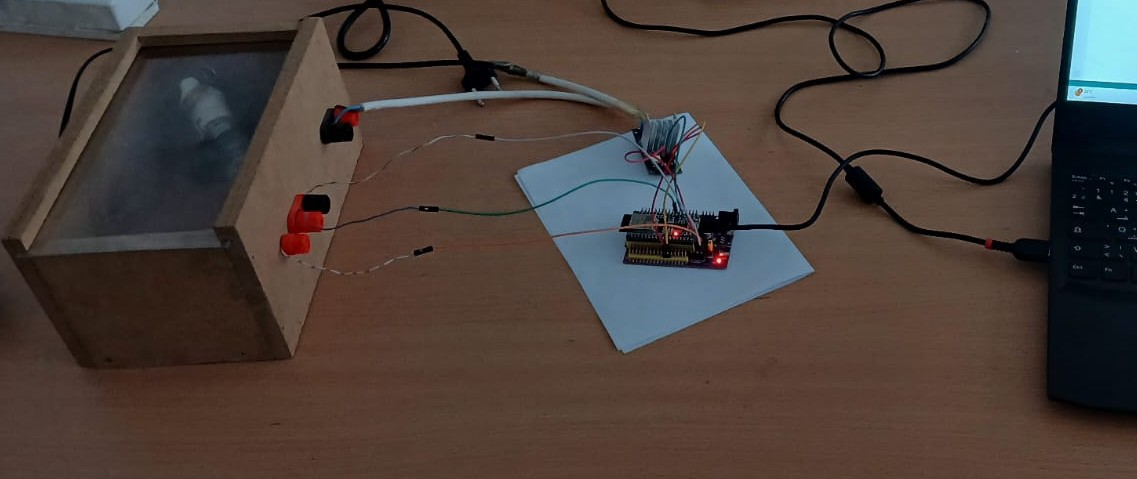
\includegraphics[width=1\linewidth]{figures/montage.jpeg}
	\caption{Montage expérimental}
	\label{fig:montage_experimental}
\end{figure}

\subsection{Déroulement de l'essai}

Après avoir mis en place le système, nous avons effectué un essai en boucle fermée. L'objectif principal de cet essai était de réguler la température en suivant une consigne donnée. Le système fonctionne en temps réel, avec une mesure de la température qui est prise toutes les 2 secondes. Pendant l'expérience, nous avons enregistré un total de 4000 échantillons afin d'analyser le comportement du système sur une durée suffisante.

Les valeurs mesurées, qui représentent les données de l'essai expérimental sur le système, telles que la température et le signal de commande, ont été récupérées à partir de la carte ESP32 et stockées dans un fichier.

\subsection{Résultats expérimentaux et analyse}

Nous avons importé les valeurs enregistrées dans MATLAB pour réaliser des simulations. Des courbes ont été tracées pour représenter l'évolution de la température et la commande. La consigne donnée est $35^\circ$C puis $45^\circ$C.

\begin{figure}[H]
	\centering
	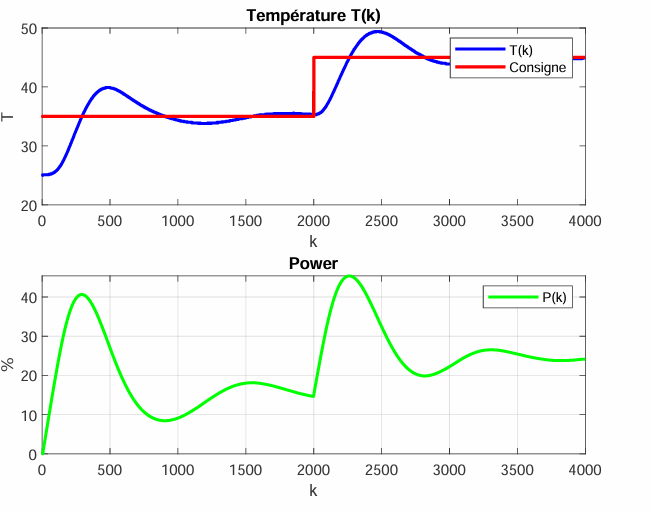
\includegraphics[width=1\linewidth]{figures/cOMMANDE8bf}
	\caption{Évolution de la sortie, de la consigne et de la commande pour l'essai en boucle fermée}
	\label{fig:commande8bf}
\end{figure}

Nous observons que la température finit par suivre correctement la consigne, ce qui montre que le système de régulation fonctionne. Cependant, cette stabilisation n'est pas immédiate, elle apparaît seulement après un certain temps de fonctionnement. De plus, on remarque la présence de petites oscillations autour de la consigne. Ces variations sont dues aux limitations du système réel, comme les délais de réponse, les perturbations externes et la nature même de la commande utilisée. Malgré ces oscillations, le système reste globalement stable et capable de maintenir la température proche de la valeur souhaitée.

\section{Communication sans fil}

\subsection{Le protocole ESP-NOW}

Nous avons utilisé le protocole \textbf{ESP-NOW} pour assurer la communication sans fil.

\textbf{ESP-NOW} est un protocole de communication sans fil développé par Espressif pour les microcontrôleurs ESP32. Il permet aux appareils d'échanger les données directement. La communication se fait sur la bande de fréquence 2,4 GHz, avec une latence très faible, de l'ordre de la milliseconde. Cela le rend très utile pour notre système puisqu'il nécessite une réponse rapide.

\begin{table}[H]
	\centering
	\caption{Caractéristiques du protocole ESP-NOW}
	\label{tab:esp_now}
	\begin{tabular}{|l|l|}
		\hline
		\textbf{Caractéristique} & \textbf{Valeur / Description} \\
		\hline
		Fréquence & 2.4 GHz \\
		\hline
		Latence & Très faible ($\sim$ ms) \\
		\hline
		Portée & $\sim$200 m en espace ouvert \\
		\hline
		Taille max des données & 250 octets par trame \\
		\hline
		Réseau Wi-Fi requis & Non \\
		\hline
		Consommation énergétique & Très faible \\
		\hline
	\end{tabular}
\end{table}

\subsection{Implémentation des algorithmes de commandes  sur les microcontroleurs ESP32}

Dans cette étape finale, nous avons divisé l'algorithme de commande à minimum de variance sur deux cartes ESP32. L'une pour la mesure de la température et l'autre pour la commande de notre système thermique. Nous avons juste ajouté des parties dans le code pour assurer la communication entre les deux cartes à travers le protocole ESP-NOW, mais l'algorithme principal de commande à minimum de variance est le même.

\begin{figure}[H]
	\centering
\begin{tikzpicture}[
	node distance=1.2cm,
	block/.style={
		rectangle, rounded corners=4pt,
		draw=black!70, fill=gray!8,
		minimum width=4.8cm, minimum height=1.6cm,
		align=center, font=\small
	},
	arrow/.style={-{Stealth[length=2.5mm]}, thick},
	dasharrow/.style={-{Stealth[length=2.5mm]}, thick, dashed},
	]
	
	% ESP32-A (Contrôleur)
	\node[block] (espA) {
		\textbf{ESP32-Commande} \\[2pt]
		\textcolor{gray!80}{\footnotesize Calcul de la commande} \\
		\textcolor{gray!80}{\footnotesize (Réseau de neurones)}
	};
	
	% ESP32-B (Actionneur/Capteur)
	\node[block, right=5.5cm of espA] (espB) {
		\textbf{ESP32-Mesure} \\[2pt]
		\textcolor{gray!80}{\footnotesize Actionneur (TRIAC)} \\
		\textcolor{gray!80}{\footnotesize + Capteur (DHT22)}
	};
	
	% Flèche Commande (A → B) — au dessus
     \draw[dasharrow]
      (espA.east) -- node[above, font=\footnotesize] 
      {Commande $u(k)$} 
      node[below, font=\scriptsize, text=gray!70] 
      {Puissance de chauffage (\%)} 
      (espB.west);
	
	% Flèche Retour (B → A) — en dessous
	\draw[dasharrow]
	(espB.south) -- ++(0,-1.0) -| (espA.south)
	node[pos=0.25, below, font=\footnotesize] 
	{Mesure $y(k)$}
	node[pos=0.25, above, font=\scriptsize, text=gray!70]
	{Température (°C)};
	
	% Label communication
	\node[font=\scriptsize\itshape, text=gray!60,
	below=2.0cm of espA, xshift=4.5cm] 
	{$\longleftrightarrow$ Communication sans fil sur la bande  (2.4~GHz)};
	
\end{tikzpicture}
	\caption{Schéma de communication entre les deux ESP32}
	\label{fig:espnow_comm}
\end{figure}

Ce schéma montre comment les deux microcontrôleurs ESP32 échangent les données avec le protocole ESP-NOW. La carte ESP32-commande sert de contrôleur. Il commence par identifier la carte ESP32-mesure grâce à son adresse MAC unique. Ensuite, elle initialise le protocole et enregistre les fonctions de rappel qui se déclenchent automatiquement à chaque envoi ou réception de message.

La carte ESP32-commande attend la réception de la température envoyée par ESP32-mesure. Elle utilise la valeur mesurée de la température pour calculer la commande optimale, puis envoie le signal de puissance en retour.

\subsection{Montage expérimental}

Dans ce deuxième montage, nous avons ajouté seulement l'autre carte ESP32, tout le reste est le même.

\begin{figure}[H]
	\centering
	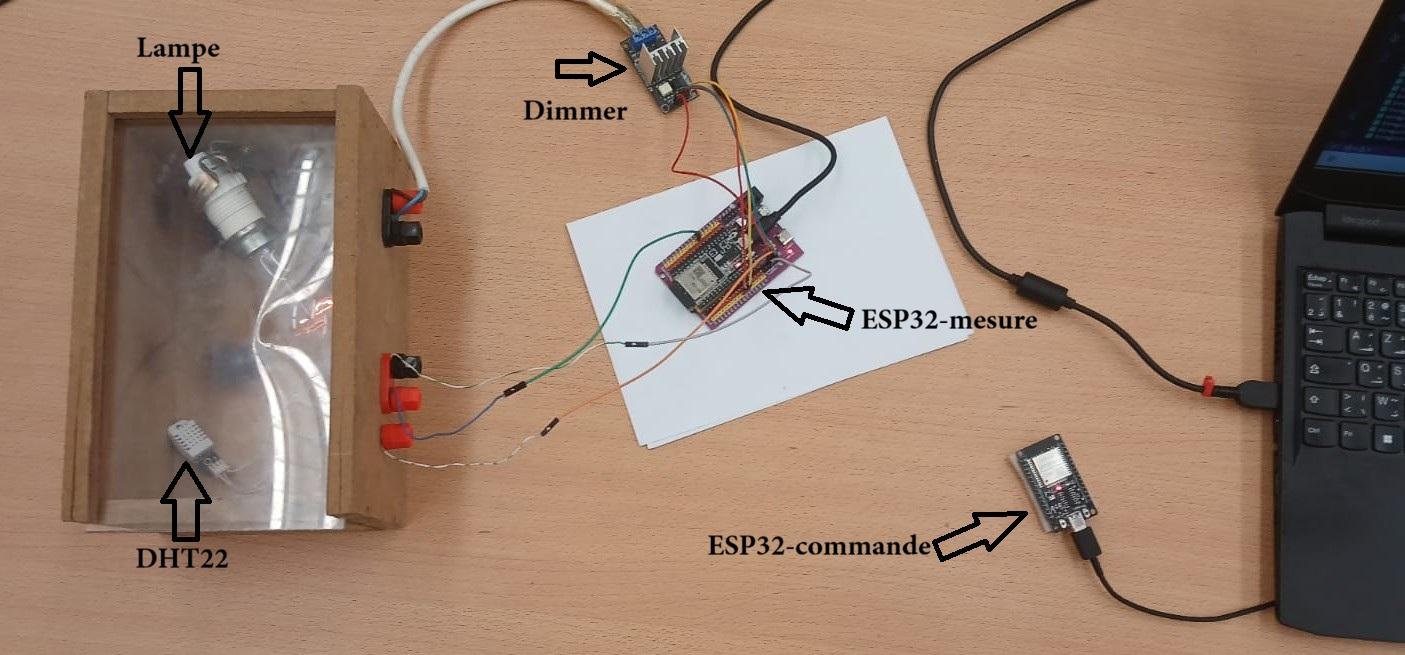
\includegraphics[width=1\linewidth]{figures/maquetttt.jpeg}
	\caption{Montage expérimental avec communication}
	\label{fig:montage_communication}
\end{figure}

\subsection{Résultats expérimentaux et analyse}

Après la mise en place du système, nous avons réalisé l'essai en boucle fermée en utilisant la communication sans fil entre les deux cartes ESP32. Au cours de cet essai, un total de 4000 mesures a été enregistré afin d'étudier le comportement du système et d'évaluer les performances de la commande dans un environnement avec communication sans fil.

Les mesures enregistrées sont importées dans MATLAB pour réaliser les simulations. La consigne donnée est $40^\circ$C et $50^\circ$C. Nous avons donc tracé les courbes suivantes.

\begin{figure}[H]
	\centering
	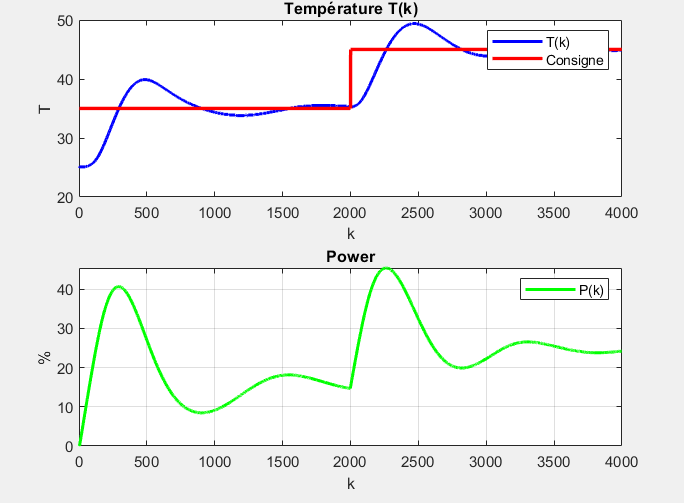
\includegraphics[width=1\linewidth]{figures/NewMann}
	\caption{Évolution de la sortie, de la consigne et de la commande}
	\label{fig:newmann}
\end{figure}

D'après les résultats obtenus, nous constatons que la température suit la consigne, mais avec un certain temps de retard. Cela signifie que le système a besoin d'un délai avant de réagir et d'atteindre la valeur souhaitée, ce qui est normal pour un système thermique à cause de son inertie. Une fois proche de la consigne, on observe la présence de petites oscillations autour de cette valeur. Ces variations sont liées aux limites du système réel et à la dynamique de la commande, mais elles restent faibles et n'affectent pas la stabilité globale. En effet, le système demeure stable et continue de fonctionner correctement.

\section*{Conclusion}

Dans ce chapitre, nous avons expliqué comment nous avons réalisé l'essai pratique de la commande à minimum de variance en commençant par l'essai expérimental sur le système pour extraire sa dynamique, et faire l'apprentissage du modèle choisi avec ses données jusqu'à arriver à faire sa commande par minimum de variance à distance en utilisant deux microcontrôleurs ESP32.

D'une part, les résultats montrent la cohérence du modèle choisi et l'efficacité de la méthode de commande introduite qui permet au système de suivre la consigne ; d'autre part, ils montrent la réponse lente des systèmes thermiques en général, ce qui ouvre des perspectives sur d'autres méthodes de commande plus efficaces pour ce type de système.